%%%%%%%%%%%%%%%%%%%%%%%%%%%%%%%%%%%%%%%%%
% a0poster Portrait Poster
% LaTeX Template
% Version 1.0 (22/06/13)
%
% The a0poster class was created by:
% Gerlinde Kettl and Matthias Weiser (tex@kettl.de)
% 
% This template has been downloaded from:
% http://www.LaTeXTemplates.com
%
% License:
% CC BY-NC-SA 3.0 (http://creativecommons.org/licenses/by-nc-sa/3.0/)
%
%%%%%%%%%%%%%%%%%%%%%%%%%%%%%%%%%%%%%%%%%

%----------------------------------------------------------------------------------------
%	PACKAGES AND OTHER DOCUMENT CONFIGURATIONS
%----------------------------------------------------------------------------------------

\documentclass[a0,portrait]{a0poster}

\usepackage{url}
\usepackage{lipsum}
\usepackage{multicol} % This is so we can have multiple columns of text side-by-side
\columnsep=100pt % This is the amount of white space between the columns in the poster
\columnseprule=3pt % This is the thickness of the black line between the columns in the poster

\usepackage[svgnames]{xcolor} % Specify colors by their 'svgnames', for a full list of all colors available see here: http://www.latextemplates.com/svgnames-colors

\usepackage{times} % Use the times font
%\usepackage{palatino} % Uncomment to use the Palatino font

\usepackage{graphicx} % Required for including images
\graphicspath{{figures/}} % Location of the graphics files
\usepackage{booktabs} % Top and bottom rules for table
\usepackage[font=small,labelfont=bf]{caption} % Required for specifying captions to tables and figures
\usepackage{amsfonts, amsmath, amsthm, amssymb} % For math fonts, symbols and environments
\usepackage{wrapfig} % Allows wrapping text around tables and figures

\usepackage[maxnames=1,backend=biber,doi=true]{biblatex}
\addbibresource{reference.bib}
% \AtEveryBibitem{%
%   \ifentrytype{article}{%
%     \clearfield{pages}%
%   }{%
%   }%
% }




\makeatletter
\renewenvironment{abstract}{%
    \if@twocolumn
      \section*{\abstractname}%
    \else %% <- here I've removed \small
        {\bfseries \Large\abstractname\vspace{\z@}}%  %% <- here I've added \Large
      \quotation
    \fi}
    {\if@twocolumn\else\endquotation\fi}
\makeatother





\begin{document}

%----------------------------------------------------------------------------------------
%	POSTER HEADER 
%----------------------------------------------------------------------------------------

% The header is divided into two boxes:
% The first is 75% wide and houses the title, subtitle, names, university/organization and contact information
% The second is 25% wide and houses a logo for your university/organization or a photo of you
% The widths of these boxes can be easily edited to accommodate your content as you see fit

\begin{minipage}[b]{0.75\linewidth}
    \veryHuge \color{NavyBlue} \textbf{FoReCo} \color{Black}\\[.5cm] % Title
\Huge\textit{A forecast-based recovery mechanism for real-time\\remote control of robotic manipulator}\\[2cm] % Subtitle
\huge \textbf{Milan Groshev, Javier Sacido \& Jorge Martín-Pérez}\\[0.5cm] % Author(s)
\huge Universidad Carlos III de Madrid\\[0.4cm] % University/organization
\huge Telcaria Ideas S.L.\\[0.4cm] % University/organization
\Large \texttt{mgroshev@pa.uc3m.es}\\ % --- 1 (000) 111 1111\\
\end{minipage}
%
\begin{minipage}[b]{0.25\linewidth}
\color{DarkSlateGray} % DarkSlateGray color for the rest of the content
    
\includegraphics[width=15cm]{logo-uc3m.eps}
    \hspace*{2cm}
\includegraphics[width=10cm]{logo-telcaria.eps}\vspace{1cm}
    \hspace*{5cm}
\includegraphics[width=5cm]{qr.eps}\\
    \hspace*{3.31cm}\large \textbf{arXiv:2205.04189}\\[0.1cm]
\end{minipage}

\vspace{1cm} % A bit of extra whitespace between the header and poster content







%----------------------------------------------------------------------------------------
%	ABSTRACT
%----------------------------------------------------------------------------------------
\color{DarkSlateGray} % DarkSlateGray color for the rest of the content
\section*{Abstract}
This demonstration presents FoReCo~\cite{foreco},
    a solution to recover lost control
    commands in remotely controlled
    robots. In the demonstration,
    visitors use a joystick to remotely
    control a robotic arm under the
    presence of packet losses in the wireless medium. The lost
    control commands result in a distorted trajectory of the robotic arm,
    thus, we deploy
    FoReCo to recover lost
    control commands using an ML model
    that we train with a real-world dataset. The demonstration shows how FoReCo recovers the lost commands, and how the robot arm operates smoothly despite the losses that are present in the wireless medium.



%----------------------------------------------------------------------------------------

\begin{multicols}{2} % This is how many columns your poster will be broken into, a portrait poster is generally split into 2 columns


% \color{Navy} % Navy color for the abstract
\color{DarkSlateGray} % DarkSlateGray color for the rest of the content


%% %----------------------------------------------------------------------------------------
%% %	INTRODUCTION
%% %----------------------------------------------------------------------------------------
%% 
%% %\color{SaddleBrown} % SaddleBrown color for the introduction
%% \color{DarkSlateGray} % DarkSlateGray color for the rest of the content
%% 
%% 
%% \section*{Introduction}
%% \label{sec:intro}
%% 
%% % Remote control I4.0, 99.999% & losses consequences
%% Real-time remote control of robotic manipulators is
%% of high interest for industry~4.0 use cases,
%% since it reduces costs and the exposure of
%% operators to hazard situations.
%% However, the presence of packet losses in
%% the the network lead to trajectory deviations
%% that prevent the robot from achieving
%% the expected 99.9999\% reliability.
%% % SoA
%% The mechatronics and robotic community
%% propose to overcome the lost/delayed 
%% control commands using time domain
%% passivity-based~\cite{TDPC-3}, and
%% wave-variable passivity-based~\cite{wvbc-4}
%% approaches that assume constant
%% network delays~\cite{TDPC-5},
%% or delays with small 
%% variability~\cite{TDPC-3,wvbc-4}.
%% Such assumptions on the network delay
%% do not apply for robots connected using
%% IEEE~802.11 wireless technology,
%% which suffers from uncontrolled
%% packet losses and delays. Specially
%% in industrial scenarios with electromagnetic
%% interference jamming the wireless channel.





%----------------------------------------------------------------------------------------
%	FoReCo
%----------------------------------------------------------------------------------------




\section*{FoReCo \& remote control}
\label{sec:foreco}

% What we propose + what it does
FoReCo~\cite{foreco} does not make assumptions on the network
delays and infers the commands that did not arrive
at the expected 150ms frequency.
FoReCo infers the lost commands with a
multinomial regression that takes as \textbf{input}:
\begin{enumerate}
    \item the \textbf{position} of each joint $j_i(t), \forall i$;
    \item for \textbf{how long} each joint has
    been moving without stopping\\
    $\max_{t_0<t}\left\{t-t_0:\ j_i(\tau)>0, \forall\tau\in[t_0,t]\right\},\ \ \forall i$; and
    \item the \textbf{angular derivative} of each joint $\tfrac{d}{d\alpha}j_i(t), \forall i$.
\end{enumerate}
Using the input (1)-(3),
FoReCo runs the multinomial logistic
regression and \textbf{outputs}
if the lost command
was an \textbf{up/down} movement,
a \textbf{righ/left} sweep, 
or a \textbf{grab/release} action.
%% The repetitive pick-and-place task
%% fosters FoReCo's accuracy
%% when it forecasts lost remote
%% control commands.



\begin{center}\vspace{1cm}
    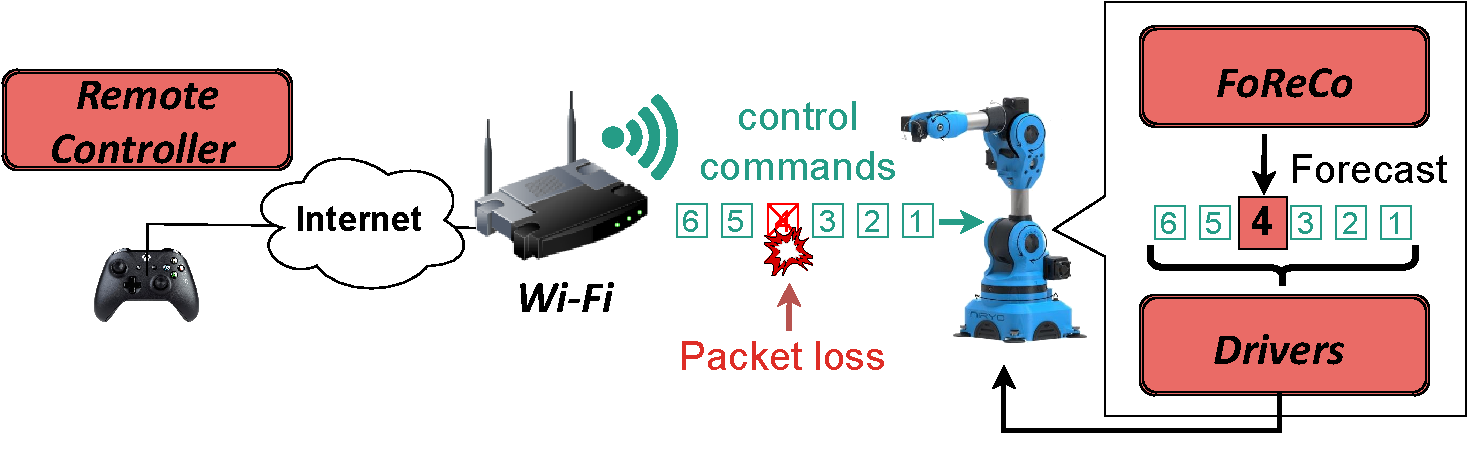
\includegraphics[width=\linewidth]{figures/experimental-setup-standalone.pdf}
    \captionof{figure}{FoReCo infers control commands lost
    in connection between the remote controller
    and the robotic arm.}
    \label{fig:foreco}
\end{center}\vspace{1cm}

%% Remote control
%% commands in factory floors are typically
%% repetitive actions as pick-and-placing
%% boxes. FoReCo exploits
%% 
%% FoReCo relies
%% on the repetitive nature of robot manipulator
%% tasks, such as pick and place tasks in a
%% production lane. Remote control commands lost
%% during repetitive tasks are easy to
%% infer/forecast if they do not arrive on time.
%% Thus, we use FoReCo to forecast/infer the
%% remote control command that does not arrive on
%% time.
%% {\color{red}In this demonstration we proof
%% that FoReCo correctly recovers
%% remote control commands
%% that are lost due to IEEE~802.11 packet
%% losses/delays in between a router and a robotic
%% arm communication.
%% In the demonstration we also show that
%% FoReCo can be integrated in end-to-end
%% Industry~4.0 platforms, namely, we use
%% DEEP~\cite{deep} to deploy a train FoReCo.}



%% %----------------------------------------------------------------------------------------
%% %	Impact of losses
%% %----------------------------------------------------------------------------------------
%% 
%% \section*{Lost/delayed control commands deviate the trajectory}
%% Although occasional command losses may be
%% irrelevant, they actually play a key role
%% in the distortion of the robot trajectory
%% as it is remotely controlled~\cite{5g-acias}. Either
%% control commands are lost or do not arrive
%% at the expected frequency, this leads to
%% the trajectory error illustrated in
%% Figure~\ref{fig:trajectory-error}.
%% 
%% \begin{center}\vspace{1cm}
%%     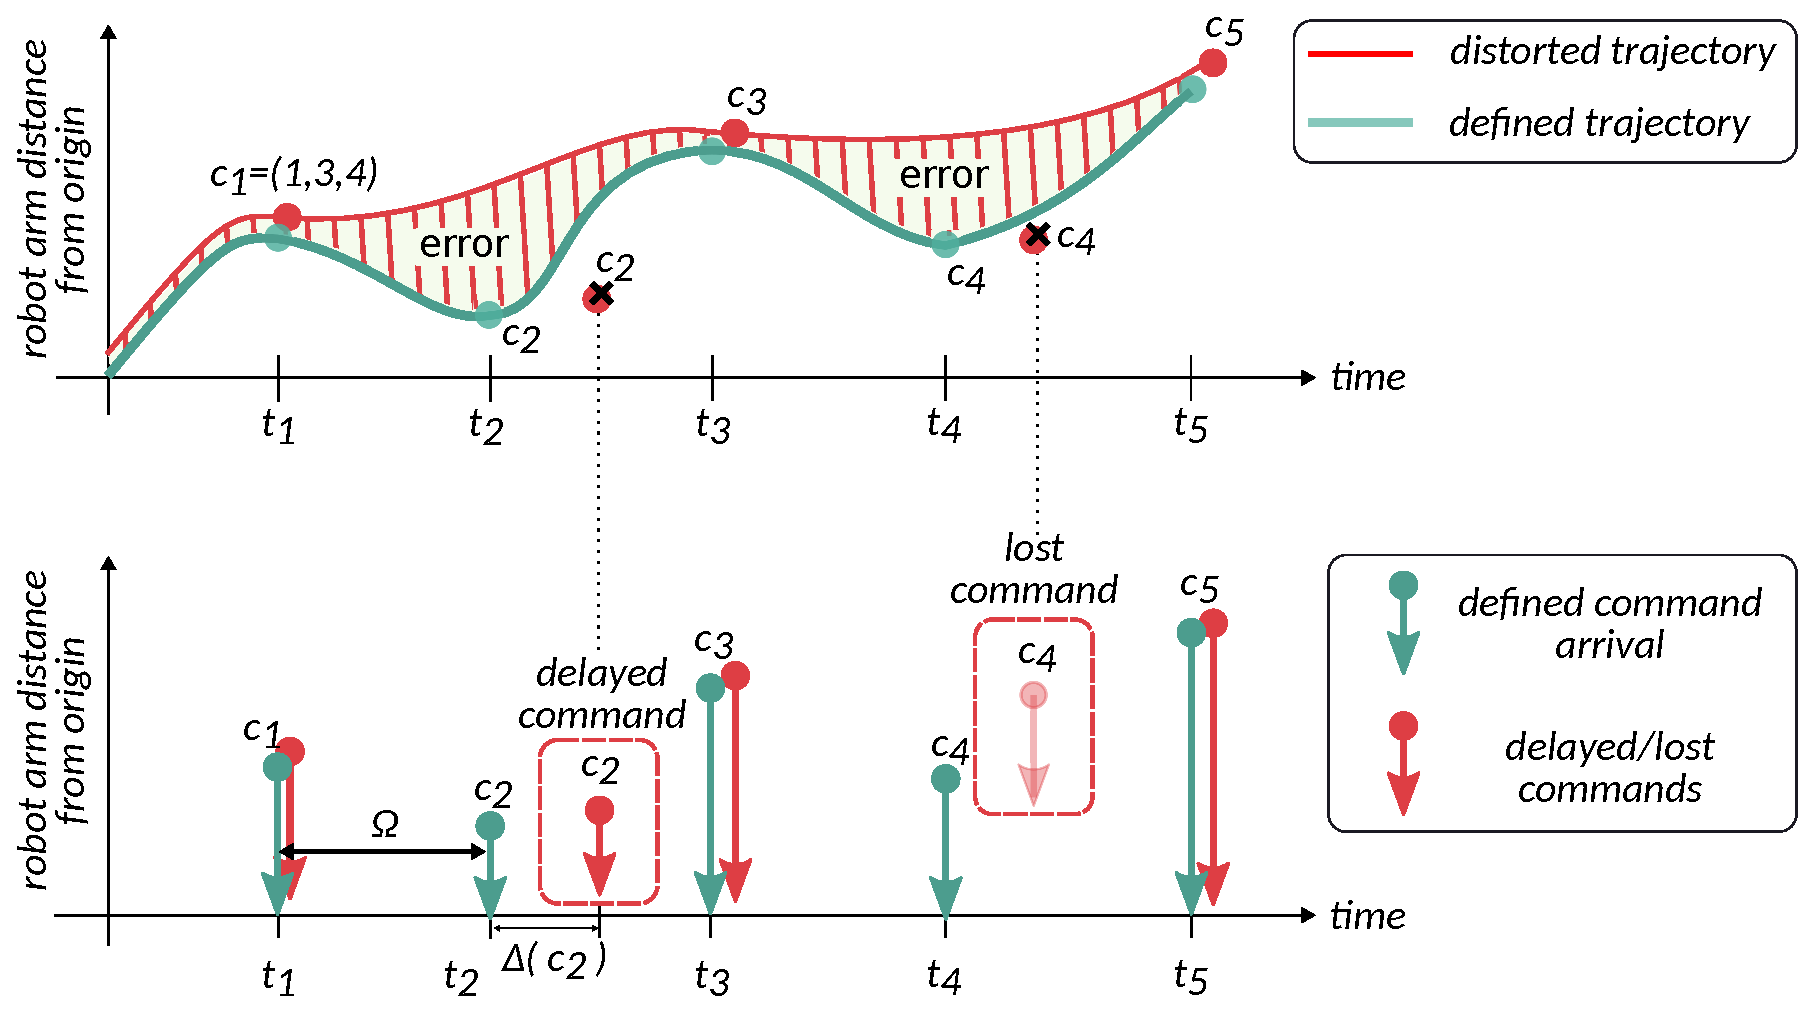
\includegraphics[width=.84\linewidth]{figures/foreco-problem-statement-two-lines.eps}
%%     \captionof{figure}{Impact of delayed and lost commands in the robot trajectory.}
%%     \label{fig:trajectory-error}
%% \end{center}\vspace{1cm}





%----------------------------------------------------------------------------------------
%	FoReCo deployment
%----------------------------------------------------------------------------------------

%% \section*{FoReCo deployment in a real-world platform}
%% \label{sec:deep}
%% 
%% FoReCo is ready to be deployed in real-world
%% platforms as DEEP/IEES~\cite{deep}
%% (see Figure~\ref{fig:setup})
%% to benefit from their monitoring, 
%% training, and automation functionalities.

%% % How we pack FoReCo for DEEP
%% In order to deploy FoReCo we create
%% a Network Service (NS) with six
%% Virtual Network Functions (VNFs)
%% illustrated as red boxes
%% in Figure~\ref{fig:setup}:
%% (1) the \textbf{FoReCo} VNF to assess the command
%% recovery;
%% (2) the robot \textbf{drivers} VNF
%% % are low-level software interfaces that
%% to control and monitor the robotic arm hardware;
%% (3) the \textbf{niryo-one-interface} and (4) \textbf{niryo-one-motion} to provide high-level abstraction for the core robot functionalities; (5) the \textbf{niryo-one-web} VNF to provide a set of tools (e.g., web interface, joystick/automated robot control, calibration) that facilitate the user interaction with the robot; and
%% (6) the \textbf{niryo-ros-master} as a central
%% entity to coordinate the communication among VNFs.
%% The niryo-one-web/interface/motion/master and the
%% drivers VNFs are implemented using
%% the Robot Operating System
%% (ROS)%~\cite{ros},
%% and the FoReCo VNF is implemented
%% using 
%% scikit-learn%~\cite{scikit-learn}
%% to forecast/infer lost commands.
%% The resulting NS with the aforementioned VNFs is deployed on top of a joint fog05/Kubernetes cluster where the robot drivers VNF is deployed as a ROS native app using fog05. The niryo-one-web/interface/motion/master are deployed as containers using Kubernetes.



%% % FoReCo is packed, lets deploy it!
%% We use the DEEP platform~\cite{deep} 
%% to train FoReCo multinomial regression, deploy it,
%% do life-cycle management, and termination. While the BASS module of the DEEP simplifies and automates the creation and management of the  NS by being the logical entry point for the user, the IESS module facilitates the training and provisioning of FoReCo by providing an intent-driven approach and AutoAI solutions.
% The deployment through
% the DEEP platform proofs that FoReCo
% is ready to be integrated in real
% world platforms.


%\begin{table}[!ht]
%\centering
%\caption{Training and inference times in different equipment}
%\label{tab:training-and-inference-comparison}
%\end{table}





%%% %----------------------------------------------------------------------------------------
%%% %	RESULTS 
%%% %----------------------------------------------------------------------------------------
%%% 
%%% \section*{Results}
%%% 
%%% Donec faucibus purus at tortor egestas eu fermentum dolor facilisis. Maecenas tempor dui eu neque fringilla rutrum. Mauris \emph{lobortis} nisl accumsan. Aenean vitae risus ante.
%%% %
%%% \begin{wraptable}{l}{12cm} % Left or right alignment is specified in the first bracket, the width of the table is in the second
%%% \begin{tabular}{l l l}
%%% \toprule
%%% \textbf{Treatments} & \textbf{Response 1} & \textbf{Response 2}\\
%%% \midrule
%%% Treatment 1 & 0.0003262 & 0.562 \\
%%% Treatment 2 & 0.0015681 & 0.910 \\
%%% Treatment 3 & 0.0009271 & 0.296 \\
%%% \bottomrule
%%% \end{tabular}
%%% \captionof{table}{\color{Green} Table caption}
%%% \end{wraptable}
%%% %
%%% Phasellus imperdiet, tortor vitae congue bibendum, felis enim sagittis lorem, et volutpat ante orci sagittis mi. Morbi rutrum laoreet semper. Morbi accumsan enim nec tortor consectetur non commodo nisi sollicitudin. Proin sollicitudin. Pellentesque eget orci eros. Fusce ultricies, tellus et pellentesque fringilla, ante massa luctus libero, quis tristique purus urna nec nibh.
%%% 
%%% Nulla ut porttitor enim. Suspendisse venenatis dui eget eros gravida tempor. Mauris feugiat elit et augue placerat ultrices. Morbi accumsan enim nec tortor consectetur non commodo. Pellentesque condimentum dui. Etiam sagittis purus non tellus tempor volutpat. Donec et dui non massa tristique adipiscing. Quisque vestibulum eros eu. Phasellus imperdiet, tortor vitae congue bibendum, felis enim sagittis lorem, et volutpat ante orci sagittis mi. Morbi rutrum laoreet semper. Morbi accumsan enim nec tortor consectetur non commodo nisi sollicitudin.
%%% 
%%% \begin{center}\vspace{1cm}
%%% 
\includegraphics[width=0.8\linewidth]{placeholder}
%%% \captionof{figure}{\color{Green} Figure caption}
%%% \end{center}\vspace{1cm}
%%% 
%%% In hac habitasse platea dictumst. Etiam placerat, risus ac.
%%% 
%%% Adipiscing lectus in magna blandit:
%%% 
%%% \begin{center}\vspace{1cm}
%%% \begin{tabular}{l l l l}
%%% \toprule
%%% \textbf{Treatments} & \textbf{Response 1} & \textbf{Response 2} \\
%%% \midrule
%%% Treatment 1 & 0.0003262 & 0.562 \\
%%% Treatment 2 & 0.0015681 & 0.910 \\
%%% Treatment 3 & 0.0009271 & 0.296 \\
%%% \bottomrule
%%% \end{tabular}
%%% \captionof{table}{\color{Green} Table caption}
%%% \end{center}\vspace{1cm}
%%% 
%%% Vivamus sed nibh ac metus tristique tristique a vitae ante. Sed lobortis mi ut arcu fringilla et adipiscing ligula rutrum. Aenean turpis velit, placerat eget tincidunt nec, ornare in nisl. In placerat.
%%% 
%%% \begin{center}\vspace{1cm}
%%% 
\includegraphics[width=0.8\linewidth]{placeholder}
%%% \captionof{figure}{\color{Green} Figure caption}
%%% \end{center}\vspace{1cm}

%----------------------------------------------------------------------------------------
%	Results
%----------------------------------------------------------------------------------------

%\color{SaddleBrown} % SaddleBrown color for the conclusions to make them stand out
\color{DarkSlateGray} % DarkSlateGray color for the rest of the content


\section*{FoReCo results}
%% \subsection*{decrease error by a 95\%}
%% figure~\ref{fig:heatmap-error} illustrates the average
%% trajectory deviation of a simulated scenario~\cite{foreco}
%% with 25 robot manipulators with/without foreco
%% as they are remotely controlled in a factory floor.
%% 
%% \begin{center}\vspace{1cm}
%%      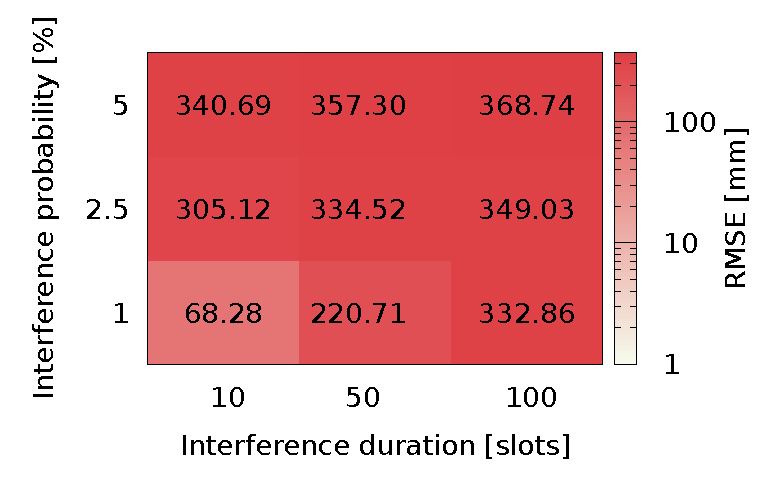
\includegraphics[width=.48\linewidth]{figures/soa-forecasts-rmse-heatmap-data-25-stas.eps}%
%%      \hfill%
%%      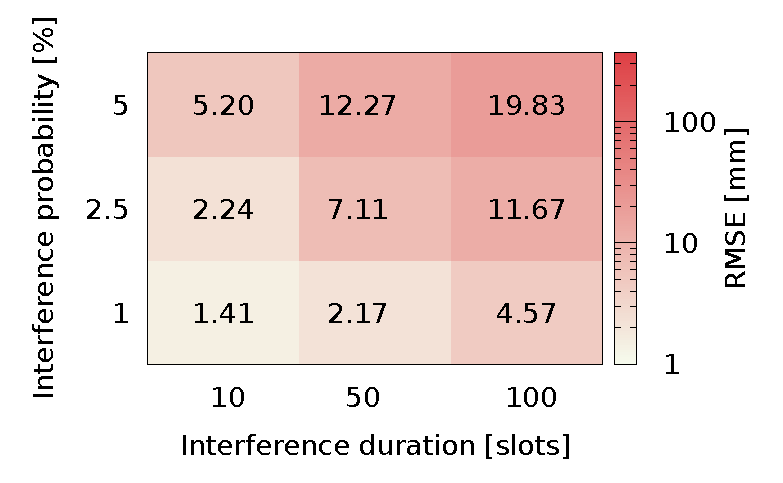
\includegraphics[width=.48\linewidth]{figures/foreco-forecasts-rmse-heatmap-data-25-stas.eps}
%%     \captionof{figure}{trajectory error as the
%%     interference duration and probability increase
%%     with or without foreco (right and left).}
%%     \label{fig:heatmap-error}
%% \end{center}\vspace{1cm}
%% 
%% 
%% 
%% \subsection*{Smoothness upon losses \& interference}
On the one hand,
Figure~\ref{fig:jammer-trajectories} shows 
that FoReCo keeps a smooth trajectory
both during and after the interference.
On the other hand, Figure~\ref{fig:jammer-trajectories}
shows that the PID-based control~\cite{control-survey}
results in a ping-pong effect that
may damage the robot rotors after channel
recovery.
% Hence, FoReCo command recovery is also
% benefitial to prevent from damaging the robot rotors
% upon ping-pong effect.




\begin{center}\vspace{1cm}
    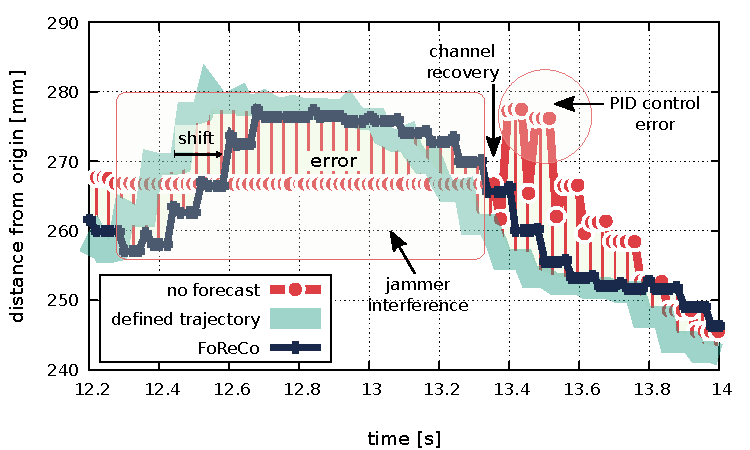
\includegraphics[width=.782\linewidth]{figures/foreco-experim-out-xyz-zoomed.pdf}
    \captionof{figure}{Robot trajectory upon IEEE 802.11 jammer interference}
    \label{fig:jammer-trajectories}
\end{center}\vspace{1cm}

\end{multicols}


%\vspace{3cm}
\section*{Demo setup}
\label{sec:setup}
In the demo setup we deploy FoReCo using the
DEEP/IESS~\cite{deep} platform to enhance the
demonstration with automation, life-cycle managament,
and model training via a GUI. This proofs that FoReCo
is ready to be deployed over real-world platforms
in industrial scenarios.

\begin{center}\vspace{1cm}
	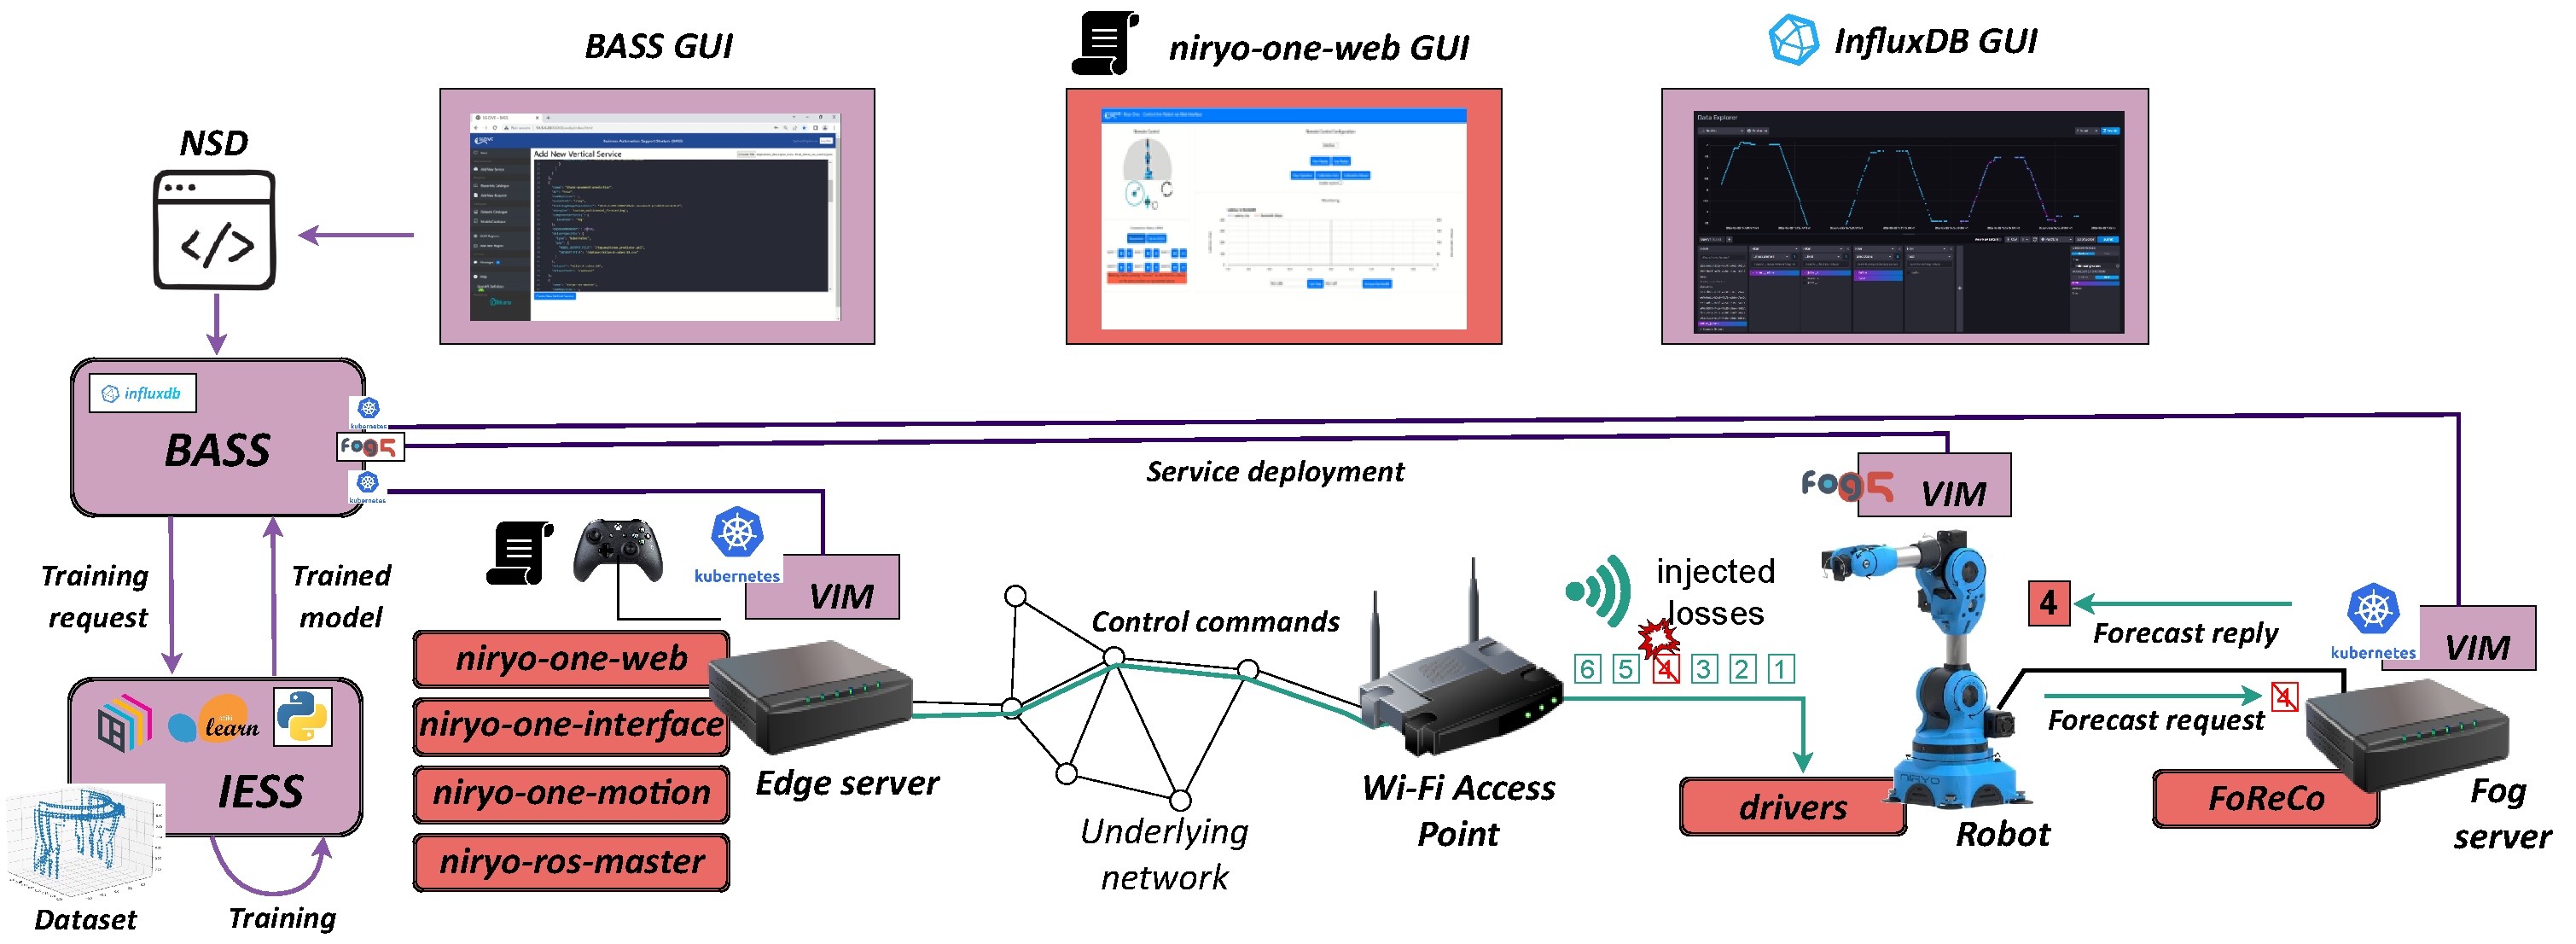
\includegraphics[width=\linewidth] {figures/experimental-setup.pdf}
    \captionof{figure}{FoReCo-assisted remote control (red) deployed with DEEP modules (purple). Three GUIs are used to deploy the service (left), calibrate/control the robot (middle), and visualize FoReCo command recovery (right).}\label{fig:setup}
\end{center}\vspace{1cm}


\color{DarkSlateGray} % Set the color back to DarkSlateGray for the rest of the content

%% %----------------------------------------------------------------------------------------
%% %	FORTHCOMING RESEARCH
%% %----------------------------------------------------------------------------------------
%% 
%% \section*{Forthcoming Research}
%% 
%% Vivamus molestie, risus tempor vehicula mattis, libero arcu volutpat purus, sed blandit sem nibh eget turpis. Maecenas rutrum dui blandit lorem vulputate gravida. Praesent venenatis mi vel lorem tempor at varius diam sagittis. Nam eu leo id turpis interdum luctus a sed augue. Nam tellus.

\begin{multicols}{2}


 %----------------------------------------------------------------------------------------
%	REFERENCES
%----------------------------------------------------------------------------------------

\printbibliography


% \nocite{*} % Print all references regardless of whether they were cited in the poster or not
% \bibliographystyle{plain} % Plain referencing style

%----------------------------------------------------------------------------------------
%	ACKNOWLEDGEMENTS
%----------------------------------------------------------------------------------------


\section*{Acknowledgements}
This work has been partly funded by the European Commission through the H2020 project Hexa-X (Grant Agreement no. 101015956), and the Spanish Ministry of Economic Affairs and Digital Transformation and the European Union-NextGenerationEU through the UNICO 5G I+D 6G-EDGEDT and 6G-DATADRIVEN.

\begin{center}%\vspace{1cm}
    
\includegraphics[width=.7\linewidth]{figures/ack-logos.png}
    \label{fig:foreco}
\end{center}%\vspace{1cm}

\end{multicols}


%----------------------------------------------------------------------------------------

%\end{multicols}

\end{document}